%\subsection{Accelerometer}
\indent Accelerometers were implemented in this package to determine the frequencies at which the element vibrates at. For lab testing, the desired data was the modal shapes of an L beam. The use of accelerometers for structural health monitoring is becoming common practice in smart bridges such as the new I-35W bridge in Minneapolis where periodic modal studies are performed\cite{Kistler}.

\subsubsection{Accelerometer Parameters}
\indent When choosing the correct accelerometer to be implemented in the sensor package, the following parameters were deciding factors:
\begin{itemize}
\item Number of Axes
\item Dynamic Range
\item Type of Mount
\item Analog vs Digital Output
\item Bandwidth
\item Power Consumption
\end{itemize}

\paragraph{Number of Axes}
\indent The number of axes decides how many directions that acceleration may be measured. Typically accelerometers have at least two axis. For the purposes of the sensor package, three axis were needed.
\paragraph{Dynamic Range}
\indent The main limiting factor for determining the proper accelerometer was the dynamic range (DR).  This refers to the range of accelerations that the sensor is capable of measuring. For a 3g accelerometer, the device can measure accelerations up to $3*9.81m/s^{2})$ (or $ 29.43 m/s^{2}$).  The value of the dynamic range is found on its corresponding data sheet.  To determine the appropriate accelerometer, the proper DR had to be determined.  This value is a dependent upon three parameters.  The equation for the dynamic range, Equation \ref{eqn:Acc_Accel} below, is dependent on the frequency being sought after and the resulting amplitude.  This equation is derived from the position function, Equation \ref{eqn:Acc_Pos};  
%Latex Code
\begin{equation}
u = Ae^{j\omega t}
\label{eqn:Acc_Pos}
\end{equation}
\begin{equation}
\dot{u} = Aj\omega e^{j\omega t}
\label{eqn:Acc_Vel}
\end{equation}
\begin{equation}
\ddot{u} = -A\omega^{2}e^{j\omega t}
\label{eqn:Acc_Accel}
\end{equation}

\noindent where $u$ is the position, $\ddot{u}$ is acceleration (or in this case the DR), \textit{A} is the displacement, $\omega$ is the measured frequency in radians, and \textit{f} is the frequency in Hertz.  This equation allows one to calculate the allowed maximum displacement before reliable data cannot be measured.  Since the frequency value of the acceleration function is squared, a change in frequency will cause a dramatic change in the maximum allowed amplitude.  Using a maximum frequency of 77.5 Hz (determined analytically by the FEM team for the simply supported beam) and a 1.5 Hz frequency (a rough representative of the Newport Bridge), the maximum displacement of a structure before unreliable data acquisition occurs was calculated for every accelerometer that was considered.  These values are shown in Table \ref{Acc_Comp_Table}.

\paragraph{Type of Mount}
\indent Accelerometers can be mounted to a circuit board in one of two manors: through-hole mounting or surface mounting.  An accelerometer with dual inline package (DIP) header pins can be placed directly into a breadboard for prototyping; whereas a surface mount accelerometer needs to be specially soldered to a PCB.
\paragraph{Analog vs Digital Output}
\indent The difference between an analog and digital accelerometer is how the output data is processed.  Analog accelerometers output a frequency that is proportional to acceleration whereas digital accelerometers output a square wave of a certain frequency.  The amount of time that the wave is high is proportional to the amount of acceleration \cite{DimensionEngineering}. 
\paragraph{Bandwidth}
\indent The bandwidth is defined as the useful frequency range in which the response falls to -3dB of the nominal value (0 Hz) \cite{MSY.SivaPrasad:2011}.  Therefore, while choosing an accelerometer, the desired frequencies must fall within the bandwidth of the sensor.   
\paragraph{Power Consumption}
\indent To conserve power, finding an accelerometer with low current draw was essential.  Fortunately most accelerometers require only a small amount of current draw.

\subsubsection{Accelerometer Selection}
\indent The comparison of the considered accelerometers is tabled below.  Initially, the AXL330 was chosen as the best option compared to the BMA220 and the ADXL362 because it is an analog accelerometer.  This is because it was determined that an analog accelerometer would allow for the easiest time synchronization of data with the other sensors.  However, during laboratory testing data was being clipped.  This data was deemed unreliable because as data is clipped the response becomes a multiple derelict function instead of a single one.  This causes data fitting to appear like a square wave instead of the intended sinusoidal wave.  Therefore the MMA7361L accelerometer was used in place of the ADXL330.  

\begin{table}[H]
    \begin{tabular}{|p{2.5cm}|p{2.5cm}|p{2.5cm}|p{2.5cm}|p{2.5cm}|p{2.5cm}|}
    \hline
    \textbf{Parameter} & \multicolumn{4}{c|}{\textbf{Accelerometer Model}}& \textbf{Units} \\
    \hline
            & BMA220 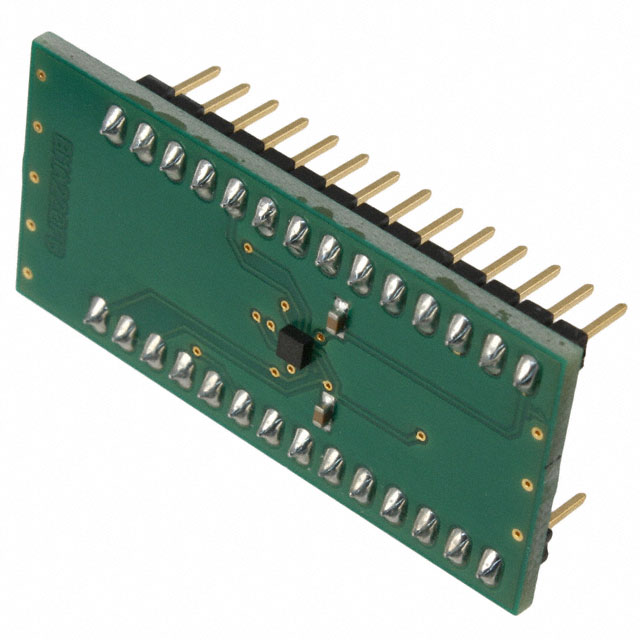
\includegraphics[width = 2.25cm ]{ACC_BMA220}    & ADXL362  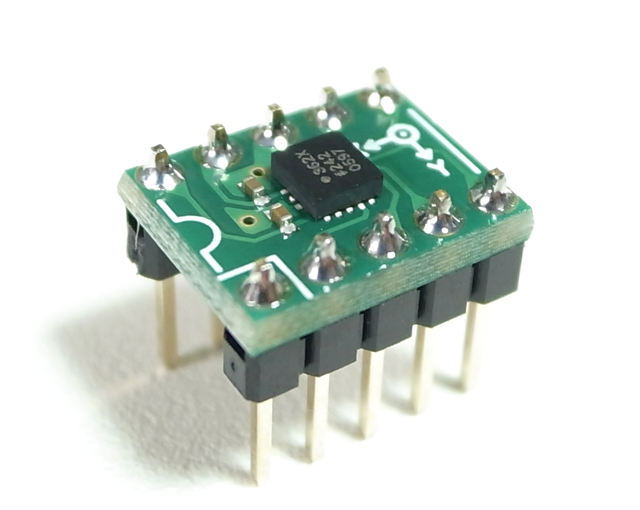
\includegraphics[width=2.25cm]{ACC_adxl362}  & ADXL330  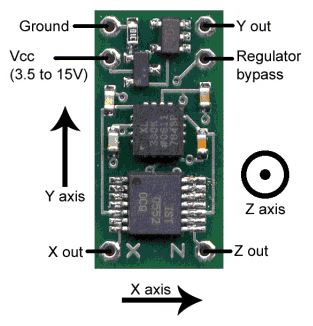
\includegraphics[width = 2.25cm ]{ACC_adxl330} & MMA7361L 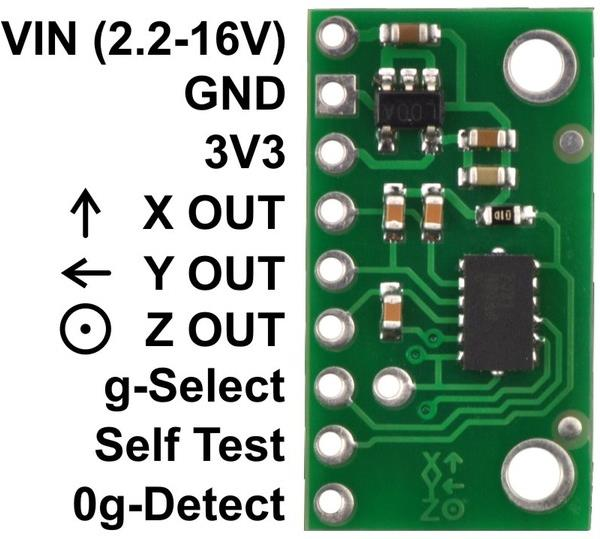
\includegraphics[width = 2.25cm ]{ACC_mma7361l} &  \\ \hline
    Analog/ {Digital}            & Digital                   & Digital            & Analog      & Analog        & ~ \\ \hline
    Dynamic Range              & $\pm$2/4/8/16g            & $\pm$2/4/8g         & $\pm$3g     & $\pm$1.5/6g   & m/s$^2$ \\ \hline
    Maximum Displacement @ 77.5 Hz & 0.083/0.165/ 0.331/0.661   & 0.083/0.165 /0.331   & 0.124       & 0.062/0.248   & mm    \\ \hline
    Maximum Displacement @ 1.5 Hz  & 220.9/441.7/ 883.5/1766.9  & 220.9/441.7/ 883.5   & 331.3       & 165.7/662.6   & mm    \\ \hline
%   \textbf{ Bandwidth}                  & ~                         & ~                   & ~           & ~             & ~     \\ \hline
    Bandwidth: X \& Y-axis               & 32/64/125/ 250/500/1000    & 50/200              & 0.5-1600    & 400           & Hz    \\ \hline
    Bandwidth: Z-Axis                     & 32/64/125/ 250/500/1000   & 50/200              & 0.5-550     & 300           & Hz    \\ \hline
    Current Draw               & 250 @ 3V           	   & 3 @ 2V   		     & 320 @ 3V    & 400 @ 3.3V    & $\mu$A     \\ \hline
    Power Consumption          & 750                       & 6                   & 960         & 1320          & $\mu$W    \\ \hline
    Number of Axes             & 3                         & 3                   & 3           & 3             & ~     \\ \hline
    \end{tabular}
    \caption{\textit{Comparison table of four accelerometers that were possible candidates for the sensor package.}}
\label{Acc_Comp_Table}
\end{table}
